\documentclass{report}

\usepackage{ucs}
\usepackage[utf8x]{inputenc}
\usepackage[T1]{fontenc}
\usepackage[french]{babel}
\usepackage{graphicx, fancyhdr, fancyvrb, hyperref, lastpage, listings, xcolor, textcomp}

\hypersetup{pdfborder = {0 0 0}}
\setlength{\headheight}{60.45229pt}

\begin{document}

\pagestyle{fancy}
\renewcommand\headrulewidth{.2pt}
\fancyhead[L]{Rapport de projet MusicBrainz}
\fancyhead[R]{
\includegraphics[scale=.75]{images/unicaen.png}}
\renewcommand\footrulewidth{.2pt}
\fancyfoot[C]{\textbf{Page \thepage/\pageref{LastPage}}}



\definecolor{lightpurple}{rgb}{0.85, 0.85, 0.85}

\lstset{
language=Bash,
basicstyle=\normalsize, % ou ça==> basicstyle=\scriptsize,
upquote=true,
aboveskip={1.5\baselineskip},
columns=fullflexible,
showstringspaces=false,
extendedchars=true,
breaklines=true,
showtabs=false,
showspaces=false,
showstringspaces=false,
identifierstyle=\ttfamily,
keywordstyle=\color[rgb]{0,0,1},
commentstyle=\color[rgb]{0.133,0.545,0.133},
stringstyle=\color[rgb]{0.627,0.126,0.941},
backgroundcolor=\color{lightpurple},
}




\begin{titlepage}
\centering
  {\large \textsc{Université de Caen Basse Normandie}}\\
  \textsc{Système - François Rioult}\\
\vspace{1cm}
  
\includegraphics[width=0.25\textwidth]{images/unicaen.png}
% \vspace{1cm}
\vfill
   {\LARGE \textbf{Rapport de projet MusicBrainz}} \\
\vspace{2em}
	{\large Suyin \bsc{LEFEBVRE} et Anthony \bsc{ROBIN}} \\
\vspace{1cm}
	
\includegraphics[width=0.35\textwidth]{images/musicbrainz_logo.png}\\
\vfill
  {\large\textbf{\today}}\\
\end{titlepage}


\renewcommand{\contentsname}{Sommaire}
\tableofcontents
\thispagestyle{fancy}


%%
% ------------------------------------------------------------------
% Introduction
% ------------------------------------------------------------------
%
%%
\chapter*{Introduction}
\addcontentsline{toc}{chapter}{Introduction}
\thispagestyle{fancy}
	\paragraph{}{
		Nous avons travaillé sur le projet MusicBrainz. Le but était d'afficher les titres qui avaient sucité le plus de reprises. Pour celà nous avons utilisé la base de données fournie par MusicBrainz sous forme de machine virtuelle sous VirtualBox couplée à un serveur nodeJs qui effectue les requêtes.
	}


	\begin{center}
		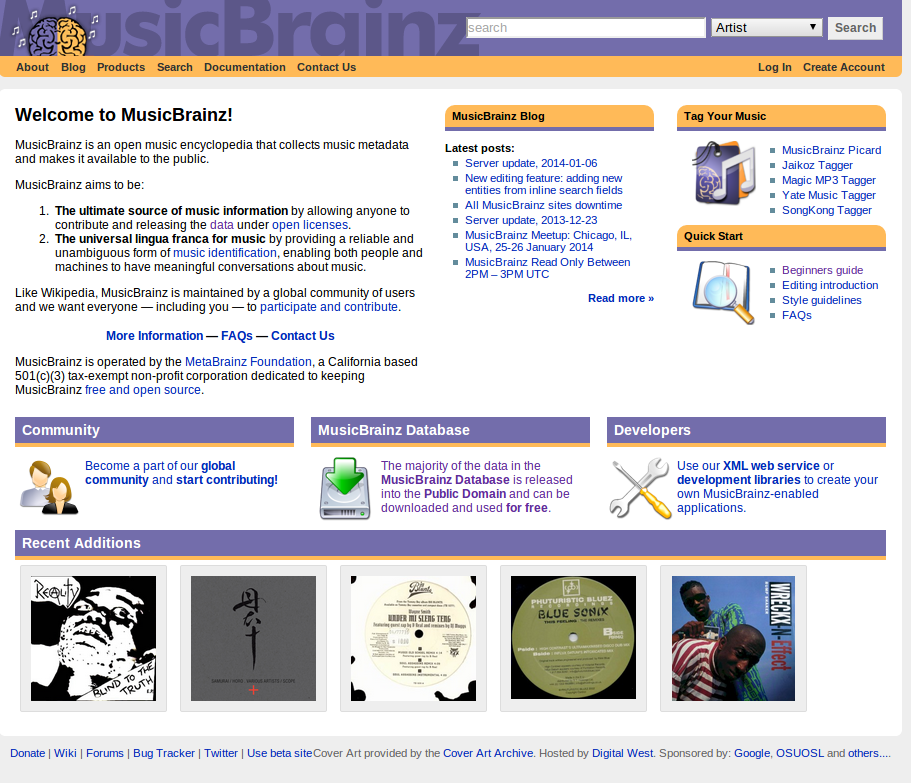
\includegraphics[width=400px]{images/homepage.png}
	\end{center}





%%
% ------------------------------------------------------------------
% Source de données
% ------------------------------------------------------------------
%
%%
\chapter*{Source de données (serveur MusicBrainz)}
\thispagestyle{fancy}
\addcontentsline{toc}{chapter}{Source de données (serveur MusicBrainz)}
	\paragraph{}{
		La source de données provient du site MusicBrainz. Nous avons téléchargé et configuré la machine virtuelle fournie.
	}


	\section*{Configurer le réseau}
	\addcontentsline{toc}{section}{Configurer le réseau}
		\paragraph{}{
			À notre domicile nous avions configuré le réseau en accès par pont, la machine avait donc sa propre adresse IP. Seulement le réseau de la faculté n’autorise pas une machine à avoir deux adresses IP. Nous n’obtenions donc plus d’adresse IPv4 pour notre machine virtuelle. Nous avons donc configuré le réseau en local uniquement.
		}

		\begin{center}
			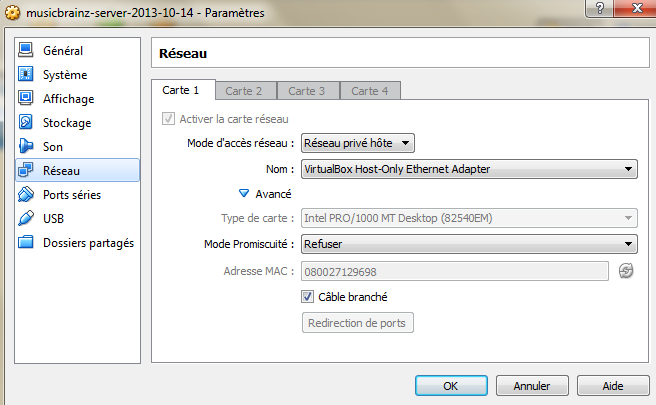
\includegraphics[scale=0.79]{images/reseau-vb.png}
		\end{center}


		\paragraph{}{
			Voici un schéma qui explique les différences entre les différentes configurations de réseau, les types de réseau VMWare sont les mêmes que ceux de VirtualBox.
		}

		\begin{center}
			\includegraphics[width=350px]{images/reseau-vmware.png}
		\end{center}


	\section*{Configurer les accès à la base de données}
	\addcontentsline{toc}{section}{Configurer les accès à la base de données}


		%%
		% ------------------------------------------------------------------
		%
		% ------------------------------------------------------------------
		%
		%%
		\subsection*{Activer l’authentification du client au serveur PostgreSQL}
		\addcontentsline{toc}{subsection}{Activer l’authentification du client au serveur PostgreSQL}

			\paragraph{}{
				L’authentification permet au serveur de la base de données d’identifier quel client est autorisé à se connecter à la base de données.
			}

			\paragraph{}{
				On édite les configurations de PostgreSql:
\begin{lstlisting}
sudo nano /etc/postgresql/9.1/main/pg_hba.conf
\end{lstlisting}

			hba signifie : « host-based authentication » c’est-à-dire  authentification fondée sur l'hôte. Chaque ligne est un enregistrement d’un type de connexion, une plage d'adresses IP (si approprié au type de connexion), un nom de base de données, un nom d'utilisateur, la méthode d'authentification à utiliser pour les connexions correspondant à ces paramètres. Nous nous servirons du format d’enregistrement suivant : host database user address auth-method
			}


			\paragraph{}{
				On ajoute la ligne :
\begin{lstlisting}
host all all 192.168.56.101/24 trust
\end{lstlisting}
				Le type de connexion host permet d’intercepter les connexions TCP/IP. La méthode d’identification trust autorise la connexion sans condition.
				On autorise ainsi tous les utilisateurs de la machine ayant l’adresse IP 192.168.56.101 (notre machine virtuelle) à se connecter à toutes les bases de données.
			}



		%%
		% ------------------------------------------------------------------
		%
		% ------------------------------------------------------------------
		%
		%%
		\subsection*{Autoriser les connexions en TCP/IP}
		\addcontentsline{toc}{subsection}{Autoriser les connexions en TCP/IP}

			\paragraph{}{
			On édite le fichier de configuration de PostgreSQL :
\begin{lstlisting}
sudo nano /etc/postgresql/9.1/main/postgresql.conf
\end{lstlisting}

			On ajouter la ligne :
\begin{lstlisting}
listen_addresses='*'
\end{lstlisting}

			Le paramètre 'listen\_addresses' indique les adresses TCP/IP sur lesquelles écoute le serveur les connexions clientes.
			On donne accès à toutes adresses IP à la base de données.
			}



		%%
		% ------------------------------------------------------------------
		%
		% ------------------------------------------------------------------
		%
		%%
		\subsection*{Redémarrer le serveur PostgreSQL}
		\addcontentsline{toc}{subsection}{Redémarrer le serveur PostgreSQL}

			\paragraph{}{
\begin{lstlisting}
sudo  /etc/init.d/postgresql restart
\end{lstlisting}

					Il faut toujours sauvegarder la machine virtuelle sinon les modifications apportées au fichier /etc/postgresql/9.1/main/postgresql.conf sont écrasées à chaque démarrage de la machine virtuelle.

			}


		%%
		% ------------------------------------------------------------------
		%
		% ------------------------------------------------------------------
		%
		%%
		\subsection*{Forcer l’adresse IP}
		\addcontentsline{toc}{subsection}{Forcer l’adresse IP}

			\paragraph{}{
				On modifie le fichier /etc/network/interfaces pour forcer l’adresse IP de la machine virtuelle sinon à chaque utilisation de la machine l’adresse IP risque de  changer.
			}

			\paragraph{}{
				On remplace:
\begin{lstlisting}
iface eth0 inet dhcp
\end{lstlisting}

				par:

\begin{lstlisting}
iface eth0 inet static
	address 192.168.56.101
\end{lstlisting}

			}


	\section*{La base}
	\addcontentsline{toc}{section}{La base}

		\paragraph{}{
			Dans la base de données MusicBrainz qui porte au total 195 tables (la commande $\backslash$dt de PostgreSQL nous renseigne cette information), nous n’utiliserons que six tables dont deux de liaisons pour notre requête qui consiste à trouver les personnes ou groupes de musique qui ont repris une chanson par rapport à son titre. Puisqu’il peut exister deux chansons qui portent le même nom, nous les différencierons grâce à l’artiste qui a écrit cette chanson.
		}

		\paragraph{}{
			Nous allons dans un premier temps chercher les chansons qui portent le titre souhaité dans la table 'work'. Un 'work' est une création intellectuelle unique, en ce sens il n’est pas forcément musical (même si c’est majoritairement le cas). Un work peut avoir plusieurs enregistrements, 'recording', ce seront nos reprises.  On trouvera donc nos reprises grâce à la table de liaison 'l\_recording\_work' où entity0 correspond au recording (reprise) et entity1 correspond au work (originale).
		}

		\begin{center}
			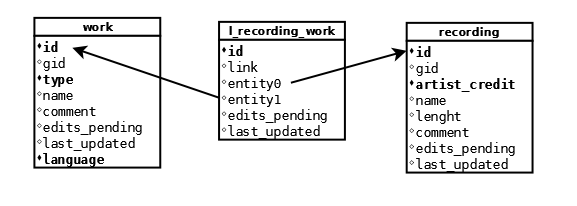
\includegraphics[scale=.5]{images/work.png}
		\end{center}


		\paragraph{}{
			Nous allons ensuite chercher le nom des artistes qui ont joués les reprises via l’attribut 'artist\_credit' et la table du même nom.
		}

		\begin{center}
			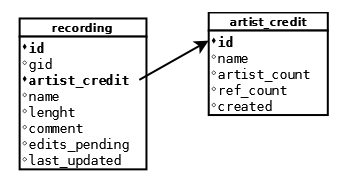
\includegraphics[scale=.5]{images/artist_credit.png}
		\end{center}


		\paragraph{}{
			Pour trouver les artistes qui ont écrit les chansons originales 'work' nous irons chercher dans la table 'artist' grâce à la table de liaison 'l\_artist\_work' où l’attribut 'entity0' correspond à l’artiste et 'entity1' correspond à la chanson.
		}

		\begin{center}
			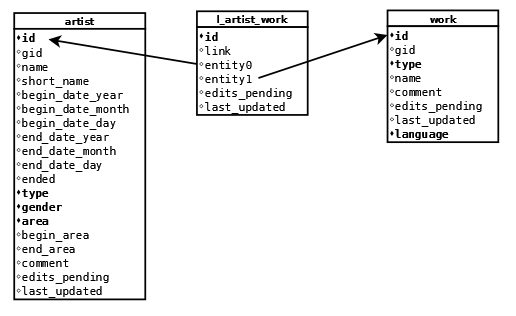
\includegraphics[scale=.8]{images/artist_work.png}
		\end{center}
		
		\paragraph{}{
			La requête est écrite en SQL. (cf. annexe \ref{requetesql})
		}



%%
% ------------------------------------------------------------------
% Serveur
% ------------------------------------------------------------------
%
%%
\chapter*{Serveur Node}
\thispagestyle{fancy}
\addcontentsline{toc}{chapter}{Serveur Node}
	\paragraph{}{
		Le serveur a été développé en nodeJs. C'est lui qui intercepte les requêtes de l'utilisateur et lui renvoie ensuite la page HTML correspondant avec les résultats.
	}

	\section*{Modules}
	\addcontentsline{toc}{section}{Modules}
		\paragraph{Express}{
			C'est un mini-framework qui va permettre de gérer plus facilement les routes (url) de notre site.
		}

		\paragraph{Ejs}{
			Ce module nous sert de moteur de template afin d'écrire notre code de la vue directement dans un fichier dédié au lieu de l'écrire dans la réponse du serveur.
		}


		\paragraph{Postgres}{
			Grâce à ce module, il est possible d'effectuer une requête sur le SGBD PostgreSQL.
		}


		\paragraph{path}{
			On spécifie le dossier contenant les ressources statiques (css, img, js) sur le serveur.
		}

		\paragraph{queryString}{
			On récupère les paramètres passés dans l'URL.
		}

		\paragraph{http}{
			Obligatoire afin d'éxecuter des requêtes au serveur. Sans lui, on ne pourrait interroger le serveur et il ne pourrait encore moins nous répondre.
		}



	\section*{Couplage à la machine virtuelle}
	\addcontentsline{toc}{section}{Couplage à la machine virtuelle}

		\paragraph{}{
		Il est impératif de spécifier le nom d'hôte de la machine virtuelle afin d'y effectuer les requêtes.\\
		L'adresse IP correspond à celle que nous avons renseigné lors de la configuration du serveur MusicBrainz.
\begin{lstlisting}
var conString = "postgres://musicbrainz@192.168.56.101:5432/musicbrainz";
\end{lstlisting}
		}



%%
% ------------------------------------------------------------------
% Auto-complétion
% ------------------------------------------------------------------
%
%%
\chapter*{Auto-complétion}
\thispagestyle{fancy}
\addcontentsline{toc}{chapter}{Auto-complétion}
	\paragraph{}{
		Du fait que l'on recherche les titres complets en base de données, nous avons choisi d'implémenter un système d’auto-complétion de titre de chanson dans la barre de recherche.
	}
	
	\paragraph{}{
		Nous avons pour cela utilisé jQuery et jQuery UI et son plugin autocomplete. \\
		Nous récupérons d'abord les caractères saisis par l'utilisateur dans le champs de recherche. Ensuite, le plugin effectue une requête ajax à l'adresse "http://musicbrainz.org/ws/2/work/?query=" en rajoutant les caractères récupérés du formulaire. \\
		Cette adresse, "http://musicbrainz.org/ws/2/work/?query=chaine+de+caracteres" nous renvoie vers un fichier xml en rapport avec "chaine de caractère". \\
		
		On parse ensuite ce fichier et l'on récupère la valeur de la balise <work> que l'on affiche dans l'autocomplete du formulaire.
	}


	\paragraph{}{
		Le plugin autocomplete que nous avons utilisé peut aussi agir directement sur un fichier XML. Nous avons donc essayé de générer un fichier depuis la base de données avec la requête:

\begin{lstlisting}
SELECT xmlforest(name) FROM work;
\end{lstlisting}

	Cette requête nous renvoie du XML du type:

\begin{lstlisting}
<name>Titre de la chanson</name>
\end{lstlisting}	
	
		Cependant, en JavaScript, nous n'avons pas réussi à écrire notre résultat dans un fichier. C'est pourquoi nous avons opté pour la solution précédente (cf fonction makeXML() dans le script serveur).		
		
	}



%%
% ------------------------------------------------------------------
% Difficultés rencontrées et Améliorations
% ------------------------------------------------------------------
%
%%
\chapter*{Difficultés rencontrées et améliorations}
\thispagestyle{fancy}
\addcontentsline{toc}{chapter}{Difficultés rencontrées et améliorations}
	\paragraph{}{
		Lors du développement de ce projet, nous nous sommes retrouvés confrontés à certaines difficultés notamment liées à la requête SQL et à la base de données.

	}
	\section*{Base de données}
	\addcontentsline{toc}{section}{Base de données}

	\paragraph{}{
		Une des premières difficultés que nous avons rencontrée est de bien comprendre la base de données, plusieurs tables ne sont pas décrites dans le schéma, les tables de liaison par exemple. Il nous a fallu tester plusieurs requêtes sur différentes tables avant de trouver la bonne. La multitude de tables nous pose alors un autre problème : le temps d'exécution de la requête.
	}
	\section*{Optimisation de la requête}
	\addcontentsline{toc}{section}{Optimisation de la requête}
	\paragraph{}{
		La requête est très longue, nous avons donc essayé de l'optimiser sans véritable succès. La fonction EXPLAIN ma\_requête permet de voir le plan de la requête (coût, utilisation d'index...)
	}
	
	\subsection*{Indexation des tables}
	\addcontentsline{toc}{section}{Indexation des tables}
	\paragraph{}{
		Nous avons tenté d'utiliser des index B-tree, le type d'index utilisé par défaut. D'après la documentation, ces index permettent de "traiter les égalités et les recherches sur des tranches de valeurs des données qui peuvent être triées". La requête s'effectue normalement plus rapidement.
		Nous avons créé des index sur les champs des tables que nous utilisions, mais cette opération n'a pas eu l'effet escompté.\\
		
		Requête SQL pour créer des index : 
		
\begin{lstlisting}
CREATE INDEX name_work_idx ON work (upper(name));
\end{lstlisting}
		
	}
	
	\subsection*{Partitionnement}
	\addcontentsline{toc}{section}{Partitionnement}
	\paragraph{}{
		Le partitionnement permet de séparer la base de données pour que celles qui ne sont pas utilisées fréquemment prennent moins de ressources. Cela permet aussi de diviser une table en sous-tables. En PostgreSQL, le partitionnement s'effectue par héritage. Nous voulions donc partionner la table "work" en tables "work\_premierLettreDuName". Chaque classe fille hérite des champs de la table mère. Ainsi selon la première lettre du titre demandé, nous allions chercher l'id dans la table fille correspondante et non dans la classe mère très conséquente. Cette amélioration n'a pas eu l'effet attendu, voir même l'effet inverse. Nous sommes donc revenu à notre requête de départ.\\
		
		Création d'une table fille :

\begin{lstlisting}
CREATE TABLE work_a(
	#nouveau champs en plus de ceux de la classe parent, si besoin
)INHERITS (work);

\end{lstlisting}
}
	\paragraph{}{
	Copie de la donnée de la classe mère vers la classe fille : 

\begin{lstlisting}
SELECT * FROM work_s (
	SELECT * FROM work
	WHERE name LIKE 'S%'
);
\end{lstlisting}

	Il faut ensuite supprimer la donnée de la table mère pour ne pas avoir de doublon.

	}

	\subsection*{Conclusion}
	\addcontentsline{toc}{section}{Conclusion}
	\paragraph{}{
		D'après ce que nous avons pu voir, nous pensons que ce sont les jointures entre plusieurs tables qui sont longues à l'exécution. Apparemment, c'est un problème courant qui est assez difficile à résoudre. Nous pourrions limiter l'utilisation de jointures dans notre requête et réaliser plusieurs requêtes plus simples. Il faudrait alors récupérer le résultat de chaque requête et les sauvegarder dans notre tableau JavaScript. Nous n'avons pas mis en pratique cette théorie.
		On pourrait peut-être aussi gérer l'affichage de la donnée différemment : ne pas attendre que la ou les requête(s) ait/aient fini de s'exécuter mais afficher quelques résultats au fur et à mesure de l'exécution.
	}
	
	\section*{Auto-complétion}
	\addcontentsline{toc}{section}{Auto-complétion}
	\paragraph{}{
		Comme vu précédemment (voir chapitre Auto-complétion), nous utilisons le site de MusicBrainz pour gérer l'auto-complétion dans notre barre de recherche. Cette utilisation a cependant une limite : l'internaute est obligé de rentrer un mot complet et faire un espace avant d'avoir accès à l'auto-complétion. Le site de MusicBrainz ne génère pas de fichier XML dans d'autres conditions. Une des améliorations possibles serait donc d'avoir ses propres fichiers XML afin de proposer une auto-complétion plus précise, au bout de trois lettres tapées par exemple. Si le fichier XML est trop lourd, nous pourrions le décomposer en plusieurs fichiers XML par rapport au trois premières lettres.
	}
%%
% ------------------------------------------------------------------
% Conclusion
% ------------------------------------------------------------------
%
%%
\chapter*{Conclusion}
\thispagestyle{fancy}
\addcontentsline{toc}{chapter}{Conclusion}
	\paragraph{}{
		Ce projet nous a permis de lier la virtual box à notre serveur nodeJS afin d'afficher la liste des reprises. Malgré une configuration de la machine virtuelle un peu laborieuse (clavier en qwerty, perte des données de config lorsque l'on éteint, ...) l'appli est fonctionnelle et nous retourne une liste des artistes ayant repris une chanson.

	}

	\paragraph{}{
		Nous avons découvert un nouveau SGBD\footnote{Système de Gestion de Bases de Données} qui fonctionne pratiquement de la même manière que MySQL. Dans ces deux SGBD les requêtes sont écrites en SQL ce qui a permis une adaptation très rapide.
	}




%%
% -------------------------------------------------------------------------
% Annexes
% -------------------------------------------------------------------------
%
%%
\appendix
\chapter{Requête SQL}
\thispagestyle{fancy}
\label{requetesql}
	\begin{lstlisting}
'WITH all_works AS ( ' +
		'SELECT * ' +
		'FROM work ' +
		'WHERE UPPER(name) LIKE UPPER(\'' + params['titre'] + '\') ' +
		')'+
	', all_recordings_works AS ( ' +
		'SELECT * ' +
		'FROM l_recording_work ' +
		'WHERE entity1 IN (SELECT id FROM all_works) ) '+
	', all_recordings AS ( '+
		'SELECT * '+
		'FROM recording '+
		'WHERE id IN (SELECT entity0 FROM all_recordings_works) ) '+
'SELECT DISTINCT (artist_credit.name, artist.name, l_recording_work.entity1) '+
'FROM artist_credit INNER JOIN all_recordings ON all_recordings.artist_credit
= artist_credit.id '+
'INNER JOIN l_recording_work ON l_recording_work.entity0 = all_recordings.id ' +
'INNER JOIN l_artist_work ON l_recording_work.entity1 = l_artist_work.entity1 '+
'INNER JOIN artist ON artist.id = l_artist_work.entity0 '+
'WHERE artist_credit.id IN (SELECT artist_credit FROM all_recordings)
	\end{lstlisting}

	\paragraph{}{
		Cette requête, à première vue complexe, comporte en réalité quatre requêtes imbriquées.

		\begin{enumerate}
		    \item recherche l'id de la chanson dans la table "work" par rapport au titre
		    \item trouve les reprises par rapport aux chansons originales
		    \item trouve l'id de l'artiste pour la reprise
		    \item trouve le nom de l'artiste des reprises et l'écrivain pour les originales
		\end{enumerate}
	}
	
	

\chapter{Base de données complète}
\thispagestyle{fancy}
		\begin{center}
			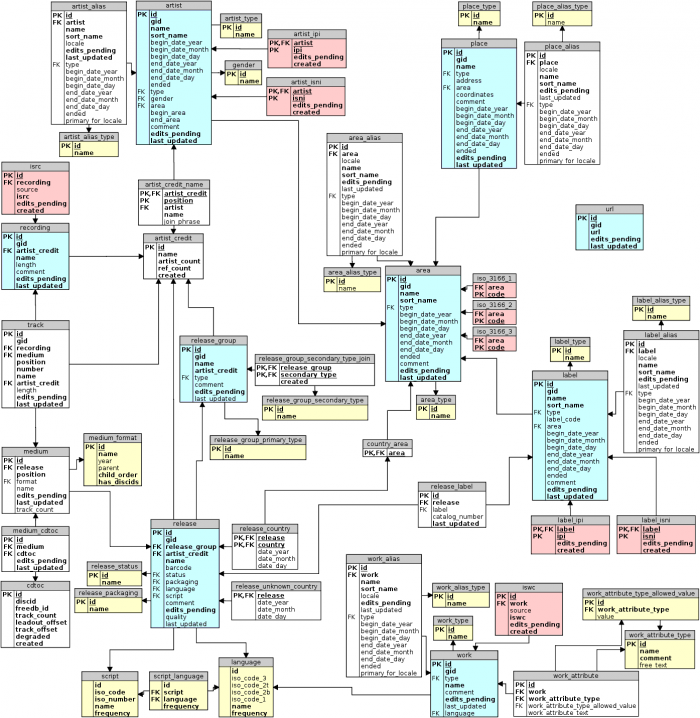
\includegraphics[scale=.5]{images/database.png}
		\end{center}






\end{document}